\documentclass[conference]{IEEEtran}
\usepackage{amsmath,amssymb}
\usepackage{graphicx}
\usepackage{booktabs}
\usepackage{multirow}
\usepackage{xcolor}
\usepackage{tikz}
\usetikzlibrary{positioning,arrows.meta,shapes.geometric,calc}
\usepackage[hidelinks]{hyperref}
\usepackage{cite}

\newcommand{\Dtwo}{\textsc{D2A}}

\begin{document}

\title{When Models Fail Silently: Detecting, Diagnosing and Adapting to Distribution Shift in Tabular Data}

\author{\IEEEauthorblockN{Team XYZ}
\IEEEauthorblockA{Rehan Farishta (Roll No. \rule{1.6cm}{0.4pt}),
Aryan Srivastava (Roll No. \rule{1.6cm}{0.4pt}),\\
Aditya Tiwari (Roll No. \rule{1.6cm}{0.4pt}),
Shivam Mishra (Roll No. \rule{1.6cm}{0.4pt})}}

\maketitle

\begin{abstract}
Machine learning models fail silently when the data they see in deployment drifts away from their training data. We study this problem on tabular data in one pipeline. A shift simulator injects six controlled shift families (covariate, noise, drift, label, concept, combined) at several severities into Adult and Covertype, and ACS Income supplies a real shift from California to four other states. We measure the damage to four standard models, reimplement the detection study of our base paper, \emph{Failing Loudly} (Rabanser \emph{et al.}, NeurIPS 2019), and extend it with \Dtwo{} (\emph{Detect--Diagnose--Adapt}). \Dtwo{} is a simple, label-free wrapper that detects a shift, diagnoses whether it is a label shift, a covariate shift or a shift to never-seen feature values, and applies the matching correction (BBSE, importance weighting or CORAL). The paper's conclusions largely transfer to tabular data: univariate KS tests match MMD, and domain classifiers need many samples. The exception is that raw features detect shift as well as the model's softmax. Every fixed correction is worse than no adaptation on average. \Dtwo{} is the only label-free method that improves all four models (up to $+1.2$ points on average, and $+6$ to $+7$ points under drift, where on Covertype it matches an oracle trained with labels). It still misses most label shifts and cannot see concept drift.
\end{abstract}

\begin{IEEEkeywords}
distribution shift, dataset shift detection, two-sample tests, label shift, covariate shift, domain adaptation, tabular data
\end{IEEEkeywords}

\section{Introduction}
A machine learning model is trained on data from one distribution and then deployed on data that keeps changing: customers age, a sensor drifts, a hospital admits a different mix of patients, or a model trained in one state is used in another. Ordinary software throws an error when its inputs are wrong; a classifier does not. It keeps producing confident predictions while its accuracy quietly falls. Rabanser \emph{et al.}~\cite{rabanser2019failing} call this \emph{failing silently} and ask how to make models \emph{fail loudly}: detect that the input distribution has changed, from as few unlabeled samples as possible, and judge whether the change is harmful.

Their study (our base paper) compares dimensionality reductions and two-sample tests on image data and finds that a simple recipe works best: feed the model's own softmax outputs into per-dimension Kolmogorov--Smirnov (KS) tests (\emph{BBSDs}). Two questions are left open, and both matter in practice. First, most real shifts are \emph{benign}~\cite{rabanser2019failing,liu2023whyshift}; an alarm on every shift is as useless as no alarm, and the paper's harm check needs labeled target data. Second, an alarm does not tell the user what to do next.

This project answers both questions on \emph{tabular} data, where most deployed models live. We (i) build a shift simulator that injects six controlled shift families at several severities into two public datasets and also use a real geographic shift (ACS Income, train on California, deploy in four other states); (ii) measure how much each shift hurts four standard models; (iii) reimplement the base paper's full detection grid on tabular data; and (iv) propose \Dtwo{} (\emph{Detect--Diagnose--Adapt}), a small wrapper around any trained classifier that, using only unlabeled target data, detects a shift, diagnoses whether it is a label shift, a covariate shift or a shift to \emph{new, never-seen} feature values, applies the matching correction (or leaves the model alone), and raises a label-free harm alarm. Every step of \Dtwo{} is a published, easy-to-explain building block; the contribution is the decision logic that connects them and an honest evaluation of it, including a design we discarded.

\section{Related Work}
\textbf{Dataset shift.} Qui\~{n}onero-Candela \emph{et al.}~\cite{quionero2009} and Moreno-Torres \emph{et al.}~\cite{morenotorres2012} give the standard taxonomy of covariate, prior (label) and concept shift. Ben-David \emph{et al.}~\cite{bendavid2010} bound target error by source error plus a divergence between domains, which explains why some shifts are harmless and others are not.

\textbf{Detecting shift.} Kernel two-sample tests based on the maximum mean discrepancy (MMD)~\cite{gretton2012mmd} and classifier two-sample tests (C2ST)~\cite{lopezpaz2017c2st} test whether two samples come from the same distribution. Lipton \emph{et al.}~\cite{lipton2018bbse} showed that, under label shift, testing the distribution of a black-box model's predictions suffices (BBSD). Rabanser \emph{et al.}~\cite{rabanser2019failing} compared all of these, plus PCA, random projections and autoencoders, and found BBSDs with univariate KS tests strongest. Out-of-distribution detection~\cite{hendrycks2017baseline} works per sample rather than per dataset, and Ovadia \emph{et al.}~\cite{ovadia2019trust} showed that model confidence degrades under shift.

\textbf{Estimating harm without labels.} Garg \emph{et al.}~\cite{garg2022atc} proposed Average Thresholded Confidence (ATC), which predicts target accuracy from the share of target predictions above a confidence threshold learned on source data. We test ATC as a label-free replacement for the base paper's labeled harm check.

\textbf{Correcting shift.} Under covariate shift, importance weighting (IW) reweights source samples by $q(x)/p(x)$~\cite{shimodaira2000}, estimated by kernel mean matching~\cite{huang2007kmm}, KLIEP~\cite{sugiyama2008kliep} or, as here, a domain classifier. Under label shift, the prior can be re-estimated by EM~\cite{saerens2002}, BBSE~\cite{lipton2018bbse} or calibrated maximum likelihood~\cite{alexandari2020mlls}. CORAL~\cite{sun2016coral} aligns second-order feature statistics. Each method assumes one shift type; \Dtwo{} picks between them automatically.

\textbf{Tabular shift benchmarks.} Folktables~\cite{ding2021folktables}, TableShift~\cite{gardner2023tableshift} and WhyShift~\cite{liu2023whyshift} provide real tabular shifts and report that most of the accuracy drop on tabular data comes from changes in $p(y\,|\,x)$ that no unlabeled method can fully fix; WILDS~\cite{koh2021wilds} plays the same role for images and text.

\section{Problem Formulation}
Let $p(x,y)$ be the source distribution and $q(x,y)$ the target distribution, with $x\in\mathbb{R}^D$ (after preprocessing) and $y\in\{1,\dots,K\}$. We observe labeled source data $\{(x_i,y_i)\}\sim p$, a classifier $f$ trained on it, and an unlabeled target sample $X_t=\{x'_j\}_{j=1}^{m}\sim q$. The three shift types are
\begin{align*}
\text{covariate:}\;& q(x)\neq p(x),\ q(y|x)=p(y|x);\\
\text{label:}\;& q(y)\neq p(y),\ q(x|y)=p(x|y);\\
\text{concept:}\;& q(y|x)\neq p(y|x).
\end{align*}
\textbf{Detection} is the two-sample test $H_0: p(x)=q(x)$ vs.\ $H_1: p(x)\neq q(x)$ at level $\alpha=0.05$. \textbf{Harm} is the accuracy drop $\Delta=\mathrm{Acc}_p(f)-\mathrm{Acc}_q(f)$; a shift is \emph{harmful} if $\Delta>\tau$ (we use $\tau=2$ points). \textbf{Adaptation} asks for a predictor $\tilde f$, built from $f$, the source data and $X_t$ only, that maximises $\mathrm{Acc}_q(\tilde f)$ and equals $f$ when no shift is detected (\emph{do no harm}). Two references bound the problem: the unadapted source model, and an \emph{oracle} retrained on labeled target data.

\section{Methodology}
Fig.~\ref{fig:pipeline} shows the whole study: the simulator produces shifted target data, the base models are scored on it, the base paper's detectors test it, and \Dtwo{} decides what to do.

\begin{figure}[t]
\centering
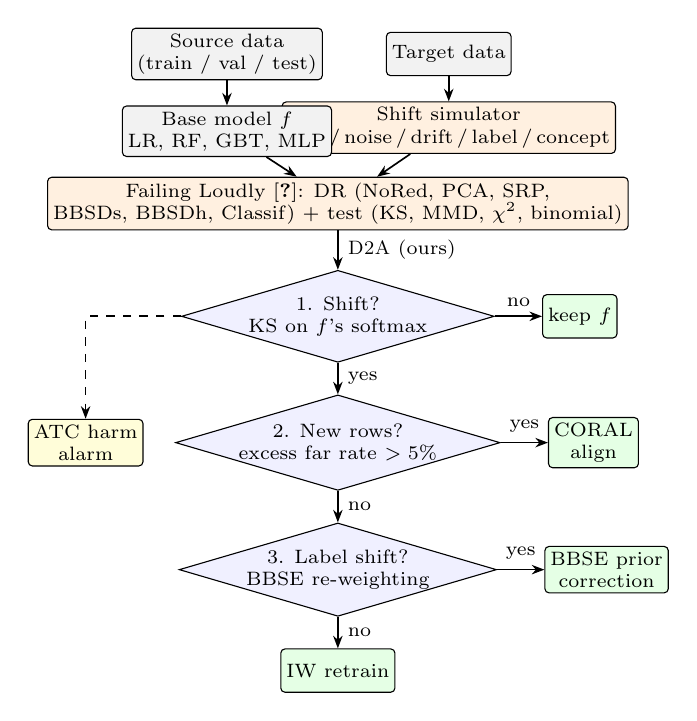
\begin{tikzpicture}[
  font=\scriptsize, node distance=3.2mm and 3mm,
  box/.style={draw, rounded corners=1.5pt, align=center, minimum height=5.5mm, inner sep=2pt, fill=#1},
  box/.default=white,
  q/.style={draw, diamond, aspect=3.4, align=center, inner sep=0pt, fill=blue!6},
  act/.style={draw, rounded corners=1.5pt, align=center, inner sep=2pt, fill=green!10, minimum height=5.5mm},
  arr/.style={-{Stealth[length=1.6mm]}, semithick}]
\node[box=gray!10] (src) {Source data\\(train / val / test)};
\node[box=gray!10, right=8mm of src] (tgt) {Target data};
\node[box=orange!12, below=of tgt] (sim) {Shift simulator\\cov.\,/\,noise\,/\,drift\,/\,label\,/\,concept};
\node[box=gray!10, below=of src] (f) {Base model $f$\\LR, RF, GBT, MLP};
\coordinate (mid) at ($(f)!0.5!(sim)$);
\node[box=orange!12, below=6mm of mid] (fl) {Failing Loudly~\cite{rabanser2019failing}: DR (NoRed, PCA, SRP,\\BBSDs, BBSDh, Classif) + test (KS, MMD, $\chi^2$, binomial)};
\node[q, below=5mm of fl] (d1) {1. Shift?\\KS on $f$'s softmax};
\node[q, below=4mm of d1] (d2) {2. New rows?\\excess far rate $>5\%$};
\node[q, below=4mm of d2] (d3) {3. Label shift?\\BBSE re-weighting};
\node[act, right=6mm of d1] (keep) {keep $f$};
\node[act, right=6mm of d2] (coral) {CORAL\\align};
\node[act, right=6mm of d3] (bbse) {BBSE prior\\correction};
\node[act, below=4mm of d3] (iw) {IW retrain};
\node[box=yellow!15, left=4mm of d2] (atc) {ATC harm\\alarm};
\draw[arr] (src) -- (f); \draw[arr] (tgt) -- (sim);
\draw[arr] (f) -- (fl); \draw[arr] (sim) -- (fl);
\draw[arr] (fl) -- node[right]{\Dtwo{} (ours)} (d1);
\draw[arr] (d1) -- node[right]{yes} (d2);
\draw[arr] (d2) -- node[right]{no} (d3);
\draw[arr] (d1) -- node[above]{no} (keep);
\draw[arr] (d2) -- node[above]{yes} (coral);
\draw[arr] (d3) -- node[above]{yes} (bbse);
\draw[arr] (d3) -- node[right]{no} (iw);
\draw[arr, dashed] (d1.west) -| (atc.north);
\end{tikzpicture}
\caption{Overview. Top: the simulator shifts the target data; base models are scored and the base paper's detectors are run on it. Bottom: our \Dtwo{} decision tree, which uses only unlabeled target data; ATC reports the estimated accuracy drop alongside.}
\label{fig:pipeline}
\end{figure}

\subsection{Shift simulator}
Each shift function takes the target pool and a severity $s$ and returns $m$ shifted rows, so the true shift type and strength are known. \emph{Covariate} shift samples rows with probability $\propto\exp(s\,z)$, where $z$ is the sum of two standardised columns (exponential tilting; $p(y|x)$ is untouched). \emph{Noise} adds Gaussian noise of $s$ column standard deviations to the numeric columns of half the rows; \emph{drift} adds a constant $s$ standard deviations instead (both move rows off the source support). \emph{Label} shift resamples rows per class to priors $(1-s)\,p(y)+s/K$. \emph{Concept} drift flips the label of rows above the median of one column with probability $s$. \emph{Combo} applies covariate then label shift. An \emph{identity} resample serves as the no-shift control.

\subsection{Base paper: Failing Loudly on tabular data}
We reimplement every representation of~\cite{rabanser2019failing} that applies to tabular data: \emph{NoRed} (standardised numeric + one-hot categorical features), \emph{PCA} and \emph{SRP} (sparse random projection) to $K=\min(32,D)$ dimensions, \emph{BBSDs} (softmax of $f$), \emph{BBSDh} (hard predictions of $f$) and \emph{Classif} (a domain classifier). Autoencoders are omitted: on 10--100 tabular features PCA already plays their role. Multi-dimensional representations are tested with one KS test per dimension, $Z=\sup_z|F_p(z)-F_q(z)|$, combined by Bonferroni (reject if $\min_k p_k<\alpha/K$), and with an MMD permutation test, $\mathrm{MMD}^2=\lVert\mu_p-\mu_q\rVert^2_{\mathcal H}$ with an RBF kernel. BBSDh uses a $\chi^2$ test on predicted-class counts; Classif trains a gradient-boosted domain classifier on half of each sample and applies a binomial test to its held-out accuracy. For harm, the paper labels the $k$ target samples the domain classifier finds most target-like and measures $f$'s accuracy on them; we use $k=100$.

\subsection{Our model: \Dtwo{} (Detect--Diagnose--Adapt)}
\textbf{Step 1: is there a shift?} The paper's best detector: KS + Bonferroni on $f$'s softmax outputs, comparing source-validation rows with the unlabeled target sample. No shift $\Rightarrow$ keep $f$.

\textbf{Step 2: does the target contain new rows?} Covariate and label shift only \emph{re-weight} rows that already exist in the source; drift, noise or a changed measurement create rows the model has never seen, and no re-weighting can fix those. We call a row \emph{far} if its nearest source-validation row is farther away than for 99\% of source rows. We compare the share of far target rows with the share a re-weighted source would have, $\sum_i w(x_i)\,\mathbb 1[x_i\text{ far}]/\sum_i w(x_i)$, using the importance weights $w$ of Step 4. If the target has more than 5 points of excess far rows, the shift is \emph{off-support} and we map target features back onto the source with CORAL~\cite{sun2016coral}, $x'=(x-\mu_t)\,\Sigma_t^{-1/2}\Sigma_s^{1/2}+\mu_s$ on standardised numeric columns, then predict with the original $f$.

\textbf{Step 3: is it a label shift?} BBSE~\cite{lipton2018bbse} estimates class weights $w_y=q(y)/p(y)$ by solving $C\,w=\hat\mu$, where $C_{ij}=\hat P_p(\hat y=i,y=j)$ is the joint confusion matrix on validation data and $\hat\mu_i=\hat P_q(\hat y=i)$. We resample source-validation rows with probability $\propto w_{y}$ and run a C2ST against the target. If the classifier can \emph{no longer} tell them apart ($p\ge\alpha$), a change of class proportions explains the shift, and we apply the BBSE prior correction $\tilde f(y|x)\propto w_y\,f(y|x)$ (no retraining).

\textbf{Step 4: otherwise, covariate shift.} A logistic-regression domain classifier $d(x)=P(\text{target}\,|\,x)$ gives importance weights $w(x)=d(x)/(1-d(x))$ ($d$ clipped to $[0.05,0.95]$), and we retrain $f$ on source data with these sample weights (IW~\cite{shimodaira2000}). IW is the \emph{safe default}: when the weights are nearly flat it reproduces $f$.

\textbf{Harm alarm.} ATC~\cite{garg2022atc} picks the confidence threshold $t$ at which the share of source-validation rows with $\max_y f(y|x)>t$ equals validation accuracy; on the target, $\widehat{\mathrm{Acc}}_q=\frac1m\sum_j\mathbb 1[\max_y f(y|x'_j)>t]$. A detected shift with $\mathrm{Acc}_{val}-\widehat{\mathrm{Acc}}_q>\tau$ raises a \emph{harmful} alarm. Our first design used this alarm as a gate (adapt only when harmful) together with an effective-sample-size rule for choosing IW vs.\ CORAL; on the development seed both proved unreliable, so we keep the gate only as an ablation (\Dtwo{}+gate). \Dtwo{} cannot see concept drift, because $q(x)$ does not change; we report this limitation rather than hide it.

\section{Datasets}
Table~\ref{tab:datasets} summarises the data. \textbf{Adult}~\cite{kohavi1996adult} (UCI census, predict income $>$\$50K; we drop the sampling weight \texttt{fnlwgt}) and \textbf{Covertype}~\cite{blackard1999covertype} (forest cover type from cartographic variables; a random 40{,}000-row subsample, 7 classes) receive simulated shifts; covariate shift tilts \texttt{age} and \texttt{education-num} (Adult) and \texttt{Elevation} and \texttt{Horizontal\_Distance\_To\_Roadways} (Covertype). \textbf{ACS Income}~\cite{ding2021folktables} (2018 American Community Survey, the modern replacement for Adult) supplies a \emph{real} shift: the model is trained on California and deployed in Wyoming, Mississippi, New York and Texas (each state capped at 40{,}000 rows). Table~\ref{tab:sample} shows sample rows of Adult.

\begin{table}[t]
\centering
\caption{Datasets (after loading; numeric / categorical features before one-hot encoding).}
\label{tab:datasets}
\setlength{\tabcolsep}{4pt}
\begin{tabular}{lrrrrl}
\toprule
Dataset & Rows & Num. & Cat. & Classes & Shift \\
\midrule
Adult & 48,842 & 5 & 8 & 2 & simulated \\
Covertype & 40,000 & 54 & 0 & 7 & simulated \\
ACS Income (CA) & 40,000 & 3 & 7 & 2 & real (state) \\

\bottomrule
\end{tabular}
\end{table}

\begin{table}[t]
\centering
\caption{Sample rows of Adult (5 of 13 features shown) with the label.}
\label{tab:sample}
\setlength{\tabcolsep}{3pt}
\begin{tabular}{rllrll}
\toprule
age & education & occupation & hours/wk & sex & label \\
\midrule
25 & 11th & Machine-op-inspct & 40 & Male & $\le$50K \\
38 & HS-grad & Farming-fishing & 50 & Male & $\le$50K \\
28 & Assoc-acdm & Protective-serv & 40 & Male & $>$50K \\
44 & Some-college & Machine-op-inspct & 40 & Male & $>$50K \\

\bottomrule
\end{tabular}
\end{table}

\section{Experimental Settings}
\textbf{Splits.} The source is split into train (50\%), validation (25\%) and test (25\%). For Adult and Covertype the source and target are two random stratified halves of the dataset, so any shift is the one we inject; for ACS they are different states. The target is split into two disjoint pools A and B, and the same shift (same random seed) is applied to both, giving $m=4000$ rows each (fewer for Wyoming). \Dtwo{} sees 1{,}000 \emph{unlabeled} rows of pool A; the oracle is trained on all of pool A \emph{with} labels; every method is scored on pool B. Preprocessing is always fitted on source-train only.

\textbf{Models.} Logistic regression (LR), random forest (RF, 200 trees), XGBoost~\cite{chen2016xgboost} gradient-boosted trees (GBT, 200 trees, depth 4, learning rate 0.1) and an MLP (64--32 hidden units, early stopping), all in scikit-learn~\cite{pedregosa2011sklearn} pipelines. GBT is the black box used by the detectors, the strongest model on average.

\textbf{Shift grid.} Covariate $s\in\{0.5,1,1.5,2,3\}$; noise and drift $s\in\{0.25,0.5,1,2\}$; label $s\in\{0.25,0.5,0.75,1\}$; concept $s\in\{0.1,0.2,0.4\}$; combo covariate $s\in\{1,2\}$ with label $s=0.5$; plus identity: 23 scenarios per dataset.

\textbf{Detection.} Target sample sizes $n\in\{10,20,50,100,200,500,1000\}$; MMD uses 100 permutations; $\alpha=0.05$. The detection rate is the share of runs with $p<\alpha$: power on shifted scenarios, false-alarm rate on identity.

\textbf{\Dtwo{}.} $\alpha=0.05$, $\tau=0.02$, excess far-row threshold $5\%$, C2ST classifier = histogram gradient boosting (100 iterations, 15 leaves), CORAL ridge $0.1$. The decision rules were designed on a separate development run (seed 0) and evaluated only on fresh seeds: \Dtwo{}'s adaptation results use seed 1 for Adult and Covertype and seeds 1--3 for ACS. Impact, detection and harm estimation do not depend on \Dtwo{}'s design, so they pool all completed runs (seeds 0--1 for Adult and Covertype, 0--3 for ACS). Everything ran on a laptop CPU. The released code also runs a larger setting (5 seeds, 8{,}000-row pools, $n$ up to 5{,}000; flag \texttt{-{}-full}); all numbers reported here come from the smaller runs above.

\section{Experiment Results and Analysis}

\begin{figure*}[t]
\centering
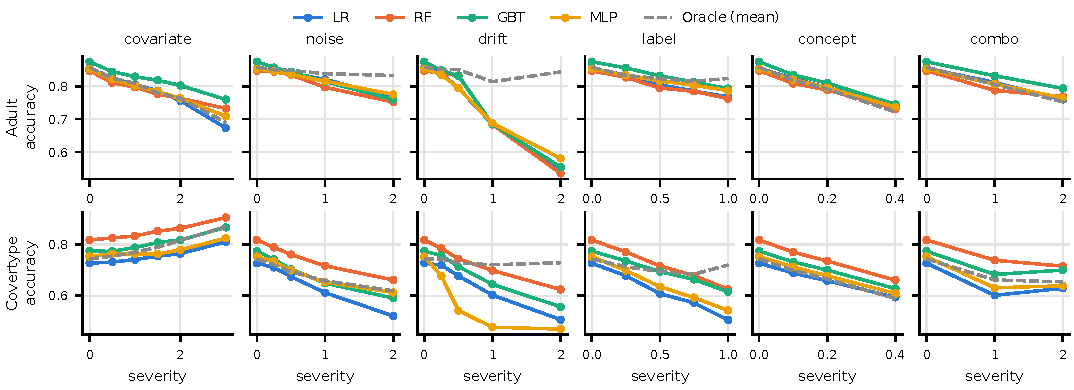
\includegraphics[width=\textwidth]{figures/fig_impact.pdf}
\caption{Impact of each simulated shift on the four base models (target-test accuracy vs.\ severity; severity 0 = no shift). Dashed: oracle retrained on labeled shifted data, averaged over models. The gap between a solid line and the dashed line is what adaptation could at best recover.}
\label{fig:impact}
\end{figure*}

\subsection{How much do shifts hurt the base models?}
Fig.~\ref{fig:impact} shows the results. Without shift, all three accuracies agree (Adult GBT: source-test 0.867, target 0.874, oracle 0.869), so the pipeline has no leakage. The shift families behave very differently:
\begin{itemize}
\item \textbf{Drift is the most damaging and the most recoverable.} At $s=2$ Adult GBT falls from 0.867 to 0.554, while the oracle still reaches 0.857. The MLP is the most fragile model (Covertype 0.469).
\item \textbf{Label shift} costs 7 points on Adult and 16 on Covertype (0.770$\to$0.615, oracle 0.724).
\item \textbf{Concept drift} hurts every model and the oracle too (Adult GBT 0.744, oracle 0.725 at $s=0.4$): no correction can recover it.
\item \textbf{Covariate shift can be benign.} On Covertype, accuracy \emph{rises} (GBT 0.770$\to$0.867 at $s=3$) because tilting toward high elevation leaves fewer, easier classes. On Adult the oracle is \emph{below} the source model (0.686 vs.\ 0.760), because the tilted target pool repeats a narrow slice of people and so carries little information.
\item \textbf{Real shift (ACS).} Every state loses accuracy. Mississippi loses most (0.810$\to$0.745, oracle 0.808); New York and Texas lose only 2 points; Wyoming loses 5 points, but its oracle (0.752, about 1{,}500 training rows) is no better.
\end{itemize}
The type of shift matters far more than the choice of model: GBT is best on Adult and RF on Covertype under almost every shift.

\begin{table}[t]
\centering
\caption{Detection rate (share of runs with $p<0.05$) over all shifted scenarios of Adult and Covertype vs.\ number of target samples $n$. Top: univariate tests; bottom: MMD.}
\label{tab:detection}
\footnotesize\setlength{\tabcolsep}{3.2pt}
\begin{tabular}{lccccccc}
\toprule
Representation (test) & 10 & 20 & 50 & 100 & 200 & 500 & 1000 \\
\midrule
NoRed (KS) & 0.33 & 0.48 & 0.65 & 0.73 & 0.76 & 0.80 & 0.85 \\
PCA (KS) & 0.31 & 0.39 & 0.59 & 0.69 & 0.76 & 0.81 & 0.84 \\
SRP (KS) & 0.35 & 0.40 & 0.65 & 0.73 & 0.78 & 0.81 & 0.83 \\
BBSDs (KS) & 0.32 & 0.38 & 0.53 & 0.59 & 0.65 & 0.78 & 0.82 \\
BBSDh (Chi2) & 0.33 & 0.38 & 0.43 & 0.55 & 0.62 & 0.68 & 0.74 \\
Classif (Binomial) & 0.00 & 0.00 & 0.38 & 0.64 & 0.74 & 0.78 & 0.83 \\
NoRed (MMD) & 0.30 & 0.39 & 0.61 & 0.68 & 0.70 & 0.78 & 0.82 \\
PCA (MMD) & 0.23 & 0.35 & 0.55 & 0.59 & 0.69 & 0.77 & 0.78 \\
SRP (MMD) & 0.25 & 0.33 & 0.55 & 0.65 & 0.67 & 0.77 & 0.80 \\
BBSDs (MMD) & 0.09 & 0.25 & 0.34 & 0.47 & 0.59 & 0.67 & 0.77 \\

\bottomrule
\end{tabular}
\end{table}

\begin{figure}[t]
\centering
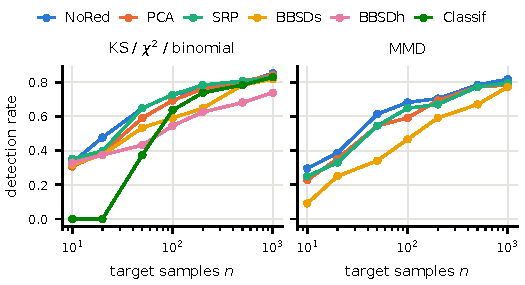
\includegraphics[width=\columnwidth]{figures/fig_detection.pdf}
\caption{Detection rate vs.\ target sample size for every representation (same data as Table~\ref{tab:detection}).}
\label{fig:detection}
\end{figure}

\subsection{Base paper on tabular data: detection}
Table~\ref{tab:detection} and Fig.~\ref{fig:detection} reproduce the paper's main comparison. Three of its findings carry over to tabular data. (i) Univariate KS tests with Bonferroni correction are as good as or better than multivariate MMD for every representation. (ii) The domain classifier is useless with few samples (0.00 at $n\le20$) but catches up at $n\ge200$ (0.83 at $n=1000$). (iii) Detection power grows steadily with $n$. One finding does \emph{not} carry over: BBSDs is not the best representation here. At $n=1000$, KS on the raw features (NoRed, 0.85) and SRP (0.83) beat BBSDs (0.82), and BBSDh is weakest (0.74). On images, dimensionality reduction is essential because the raw input has thousands of correlated pixels; tabular data has only 13--54 meaningful columns, so testing each of them directly works well. BBSDs still has a practical advantage: it ignores shifts that do not change the model's outputs, which are usually the harmless ones. False alarms on the no-shift control were mostly 0--25\% per cell (one cell 50\%). Each cell comes from only four runs, so these rates are noisy; NoRed-KS and Classif raised no false alarm at all.

\begin{table}[t]
\centering
\caption{BBSDs + KS detection rate per shift family (identity = false-alarm rate).}
\label{tab:detectshift}
\footnotesize\setlength{\tabcolsep}{3.6pt}
\begin{tabular}{lccccccc}
\toprule
Shift & 10 & 20 & 50 & 100 & 200 & 500 & 1000 \\
\midrule
identity & 0.00 & 0.25 & 0.00 & 0.00 & 0.00 & 0.25 & 0.25 \\
covariate & 0.65 & 0.75 & 0.85 & 1.00 & 1.00 & 1.00 & 1.00 \\
noise & 0.06 & 0.06 & 0.25 & 0.19 & 0.31 & 0.69 & 0.81 \\
drift & 0.31 & 0.38 & 0.69 & 0.62 & 0.75 & 0.94 & 0.94 \\
label & 0.19 & 0.38 & 0.38 & 0.62 & 0.75 & 0.94 & 1.00 \\
concept & 0.08 & 0.00 & 0.08 & 0.08 & 0.00 & 0.00 & 0.00 \\
combo & 0.62 & 0.62 & 1.00 & 1.00 & 1.00 & 1.00 & 1.00 \\

\bottomrule
\end{tabular}
\end{table}

Per shift (Table~\ref{tab:detectshift}), covariate and combined shifts are caught almost always from $n=100$; label shift and drift need about 500 samples; noise is the hardest (0.81 at $n=1000$, and only 0.25--0.46 per severity when averaged over all $n$); and concept drift is \emph{never} detected (at most 0.08, the level of false alarms). The last result is not a weakness of a particular test: under concept drift $q(x)=p(x)$, so no detector that sees only unlabeled inputs can notice it.

\begin{table}[t]
\centering
\caption{Estimating harm (GBT, all datasets): mean absolute error of the estimated target accuracy and how well ``drop $>2$ points'' is classified.}
\label{tab:malignancy}
\footnotesize\setlength{\tabcolsep}{3pt}
\begin{tabular}{lcccc}
\toprule
Estimate & MAE & Harm acc. & Harmful rec. & Benign rec. \\
\midrule
ATC (0 labels) & 0.053 & 0.578 & 0.500 & 0.846 \\
Paper top-$k$ (100 labels) & 0.061 & 0.716 & 0.711 & 0.731 \\
Random (100 labels) & 0.036 & 0.750 & 0.767 & 0.692 \\

\bottomrule
\end{tabular}
\end{table}

\begin{figure}[t]
\centering
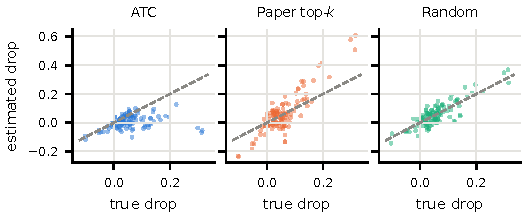
\includegraphics[width=\columnwidth]{figures/fig_malignancy.pdf}
\caption{Estimated vs.\ true accuracy drop. ATC (no labels) is compressed toward zero; the paper's top-$k$ heuristic over-estimates large drops; 100 random labels track the diagonal.}
\label{fig:malignancy}
\end{figure}

\subsection{Is the shift harmful?}
Table~\ref{tab:malignancy} and Fig.~\ref{fig:malignancy} compare three ways to judge harm. The paper's heuristic labels the 100 samples that look most target-like. It classifies harm correctly 72\% of the time, but it is biased: the most unusual samples are also the hardest, so it over-estimates large drops. Labeling 100 \emph{random} target samples is simpler, has lower error (MAE 0.036) and classifies harm better (75\%). The label-free ATC estimate has a similar average error (0.053), but it is compressed toward zero. Under drift and noise the model stays confident while being wrong, so ATC catches only half of the harmful shifts (benign recall 0.85). The practical lesson: a label-free estimate is good for a coarse alarm, and a small random labeled sample is the reliable way to confirm harm.

\begin{table}[t]
\centering
\caption{Target accuracy of GBT after adaptation (mean over severities). Adult and Covertype: held-out seed 1; ACS: seeds 1--3. Bold: best method that uses no target labels; Oracle uses them.}
\label{tab:adapt}
\footnotesize\setlength{\tabcolsep}{2.6pt}
\begin{tabular}{lcccccc}
\toprule
Data / shift & None & BBSE & IW & CORAL & \Dtwo{} & Oracle \\
\midrule
Adult / identity & 0.874 & \textbf{0.876} & 0.874 & 0.847 & \textbf{0.876} & 0.870 \\
Adult / covariate & 0.800 & 0.705 & \textbf{0.809} & 0.700 & 0.783 & 0.798 \\
Adult / noise & \textbf{0.818} & 0.809 & 0.816 & 0.799 & 0.813 & 0.846 \\
Adult / drift & 0.755 & 0.706 & 0.760 & 0.817 & \textbf{0.824} & 0.839 \\
Adult / label & 0.823 & \textbf{0.845} & 0.822 & 0.753 & 0.829 & 0.839 \\
Adult / concept & 0.793 & 0.793 & \textbf{0.794} & 0.779 & 0.793 & 0.784 \\
Adult / combo & 0.806 & 0.721 & \textbf{0.811} & 0.672 & \textbf{0.811} & 0.805 \\
Covertype / identity & \textbf{0.774} & 0.769 & 0.762 & 0.737 & \textbf{0.774} & 0.760 \\
Covertype / covariate & 0.811 & 0.777 & \textbf{0.833} & 0.539 & \textbf{0.833} & 0.808 \\
Covertype / noise & \textbf{0.675} & 0.663 & 0.672 & 0.648 & 0.653 & 0.684 \\
Covertype / drift & 0.672 & 0.642 & 0.668 & 0.730 & \textbf{0.732} & 0.729 \\
Covertype / label & 0.679 & \textbf{0.745} & 0.678 & 0.434 & 0.681 & 0.720 \\
Covertype / concept & \textbf{0.685} & 0.682 & 0.678 & 0.662 & \textbf{0.685} & 0.656 \\
Covertype / combo & \textbf{0.711} & 0.691 & 0.677 & 0.524 & 0.677 & 0.670 \\
ACS / MS & 0.747 & 0.744 & 0.733 & \textbf{0.777} & 0.740 & 0.809 \\
ACS / NY & \textbf{0.787} & 0.783 & 0.772 & 0.772 & 0.777 & 0.784 \\
ACS / TX & 0.788 & 0.780 & 0.774 & \textbf{0.795} & 0.787 & 0.793 \\
ACS / WY & 0.758 & 0.726 & 0.735 & \textbf{0.759} & 0.735 & 0.750 \\
All / mean & 0.764 & 0.748 & 0.759 & 0.708 & \textbf{0.767} & 0.775 \\

\bottomrule
\end{tabular}
\end{table}

\begin{table}[t]
\centering
\caption{Mean target accuracy over all scenarios and datasets for every base model. \Dtwo{}+gate adapts only when ATC says the shift is harmful (our first design).}
\label{tab:models}
\footnotesize\setlength{\tabcolsep}{2.4pt}
\begin{tabular}{lccccccc}
\toprule
Model & None & BBSE & IW & CORAL & \Dtwo{} & +gate & Oracle \\
\midrule
LR & 0.728 & 0.681 & 0.724 & 0.706 & \textbf{0.740} & 0.729 & 0.759 \\
RF & 0.768 & 0.743 & 0.767 & 0.731 & \textbf{0.776} & 0.776 & 0.773 \\
GBT & 0.760 & 0.742 & 0.758 & 0.699 & \textbf{0.765} & 0.760 & 0.775 \\
MLP & 0.735 & 0.705 & 0.736 & 0.718 & \textbf{0.747} & 0.741 & 0.762 \\

\bottomrule
\end{tabular}
\end{table}

\begin{figure}[t]
\centering
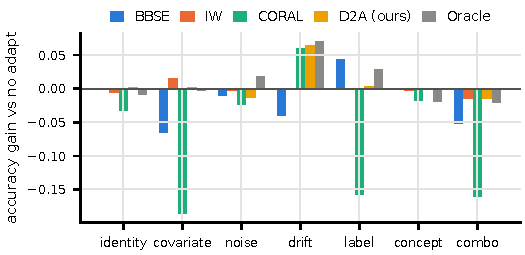
\includegraphics[width=\columnwidth]{figures/fig_adapt.pdf}
\caption{Accuracy gain over no adaptation per shift family (GBT, Adult and Covertype). Every fixed correction is harmful for some shift; \Dtwo{} follows the best one where its diagnosis is right.}
\label{fig:adapt}
\end{figure}

\subsection{Our model: \Dtwo{}}
\begin{table}[t]
\centering
\caption{Action chosen by \Dtwo{} for each true shift (\% of GBT runs).}
\label{tab:diagnosis}
\footnotesize\setlength{\tabcolsep}{5pt}
\begin{tabular}{lcccc}
\toprule
True shift & none & BBSE & IW & CORAL \\
\midrule
identity & 50 & 50 & 0 & 0 \\
covariate & 0 & 0 & 90 & 10 \\
noise & 0 & 0 & 38 & 62 \\
drift & 0 & 0 & 50 & 50 \\
label & 0 & 38 & 62 & 0 \\
concept & 83 & 17 & 0 & 0 \\
combo & 0 & 0 & 100 & 0 \\
real & 42 & 0 & 58 & 0 \\

\bottomrule
\end{tabular}
\end{table}

\textbf{Overall.} Tables~\ref{tab:adapt} and~\ref{tab:models} and Fig.~\ref{fig:adapt} compare \Dtwo{} with no adaptation, each correction applied \emph{always}, and the oracle. Every fixed correction is worse than doing nothing on average (GBT, Table~
ef{tab:adapt} mean: BBSE 0.748, IW 0.759, CORAL 0.708 vs.\ 0.764), because each one hurts badly under the wrong shift: across all models, always-CORAL loses up to 49 points in a single run and always-BBSE up to 27. \Dtwo{} is the only label-free method that beats no adaptation, and it does so for \emph{all four} base models (LR $+1.2$, RF $+0.8$, GBT $+0.5$, MLP $+1.2$ points). For RF it even slightly exceeds the oracle (0.776 vs.\ 0.773). Over all model--scenario runs, \Dtwo{} gains more than one point in 25\% of runs, loses more than one point in 19\%, and gains $+0.9$ points on average.

\textbf{Where it works.} Off-support shifts are where \Dtwo{} pays off most. Under drift it lifts Adult from 0.755 to 0.824 (oracle 0.839) and Covertype from 0.672 to 0.732, matching the oracle (0.729) without a single label. Under covariate tilt it chooses IW in 90\% of runs (Table~\ref{tab:diagnosis}) (Covertype 0.811$\to$0.833), and under combined shift it always chooses IW, the safe choice. Under concept drift it correctly does nothing in 83\% of runs.

\textbf{Where it fails.} (i) \emph{Label shift}: BBSE alone is the best fix (Adult 0.845, Covertype 0.745), but the label-shift check accepted only 38\% of label-shift runs. The C2ST is sensitive enough to reject small errors in the BBSE weights, especially for rare Covertype classes, so \Dtwo{} falls back to the harmless IW. (ii) \emph{Noise}: the off-support check fires correctly, but CORAL slightly hurts (Covertype 0.653 vs.\ 0.675), because the noise adds variance to only half of the rows while CORAL rescales all of them. (iii) \emph{Real shift}: on ACS, \Dtwo{} mostly diagnoses covariate shift and applies IW, which costs up to 2 points (Wyoming). Only CORAL helps (Mississippi $+3$ points), and the oracle gains 6, which suggests that part of the real shift is in $p(y|x)$, as WhyShift~\cite{liu2023whyshift} also reports for tabular data.

\textbf{Ablation: harm gate.} Adapting only when ATC raises the harm alarm (\Dtwo{}+gate) makes \Dtwo{} more conservative: losses fall from 19\% to 12\% of runs, but wins fall from 25\% to 13\%, and the mean gain halves ($+0.4$ points). The reason is Table~\ref{tab:malignancy}: ATC flagged only 16 of the 45 truly harmful GBT runs. A better label-free harm estimate would directly improve this trade-off.

\textbf{Effort.} \Dtwo{} adds two classifier tests, one nearest-neighbour search and at most one retraining to a deployed model, all of which take a few seconds on a laptop.

\section{Conclusion}
We built one simple pipeline that simulates distribution shift on tabular data, measures its damage, detects it with the methods of Failing Loudly~\cite{rabanser2019failing}, and handles it with our \Dtwo{} wrapper. Four lessons stand out.
(1) The \emph{kind} of shift matters more than the model: drift and label shift are harmful but recoverable, concept drift is harmful and unrecoverable without labels, and covariate shift is often harmless.
(2) The base paper's detection results mostly hold on tabular data, but there raw features are as good a representation as the model's softmax, and concept drift is invisible to every unlabeled detector.
(3) Judging harm without labels is the weak link. ATC misses half of the harmful shifts, and 100 \emph{random} labels judge harm better than the paper's most-anomalous-sample heuristic.
(4) No single correction is safe to apply blindly. A short, explainable diagnosis (``can a re-weighting explain the shift, and does it bring new rows?'') turns three individually risky fixes into a method that helps every base model, recovers drift as well as an oracle, and defaults to a harmless choice when unsure.

\textbf{Limitations and future work.} \Dtwo{}'s label-shift check is too strict, which costs most of BBSE's potential gain; a calibrated maximum-likelihood label-shift estimator~\cite{alexandari2020mlls} or a looser test level could fix this. CORAL is too blunt for noise that affects only part of the rows. On the real ACS shift no label-free fix helps much, which points to changes in $p(y|x)$; a small labeled budget, as the harm results suggest, is the natural next step. Finally, the Adult and Covertype adaptation results come from one held-out seed, and the code's larger setting (\texttt{-{}-full}) would tighten all estimates.


\bibliographystyle{IEEEtran}
\bibliography{refs}

\end{document}
